\documentclass[12pt, a4]{article}

\usepackage{booktabs}
\usepackage{hyperref}
\usepackage{float}
\usepackage{graphicx}
\usepackage{url}
\usepackage[T1]{fontenc}
\usepackage{babel}
\usepackage[utf8]{inputenc}

\graphicspath{{./images/}}

\title{The effect of color on performance in logic-based tasks}
\author{Igor Krzywda}

\begin{document}
\maketitle

\section*{Introduction}

\subsection*{Aim of the experiment}
The aim of this experiment is to find out how color (IV) might affect cognitive performance (DV).  

\subsection*{Relevance of the experiment}
The knowledge on how color affects cognitive performance can be greatly leveraged by any field that holds great value in productivity and mental performance. 
One such example could be schools, where the focus plays key role in taking in new information by students. Ranging from the color of classrooms to mindful choices of
colors used in textbooks may have compounding effect on efficiency of teaching and learning. The applications reach far further than school alone, because many jobs 
are based around intellectual work, so being mindful of color choices might pay off in increase in overall productivity of a company. On an individual level, this 
could mean more accurate choices of colors for different rooms with different uses.

\subsection*{Theory behind the experiment}
The experiment itself is one of six experiments exploring the impact of red color general performance done by Elliot, Maier, Moller, Friedman and Meinhardt and published in 
2007. Many of existing reseaches on the topic of the impact of color on performance have been done to find ways to improve cognitive and athletic performance through manipulating
colors, examples of such studies could be one of Rosenstein from 1985 exploring the effect of the color of environment on task performance and mood in people with varying SAT 
scores. There were also theoretical studies which were based on idea derived from a hypothesis proposed by Goldstein in 1942 which stated that human body has hard-wired 
physiological responses to colors. Longer wavelength (warmer) colors, like red, are said to be stimulating and directing focus on the environment, whereas shorter wave colors
(colder), like blue, are calming and direct the focus inwards. This hypothesis combined with Yerkes-Dodson law, which states that there is an optimal level of stimulation for 
maximum performance in a task. So in the context of this study, manipulating colors is a mean to control the level of stimulation coming from the environment.

\subsection*{Variables and hypotheses}
The research aims to explore the effect of color on cognitive performance. The independent variable, which is color, is operationalized into the color of participant number
on the task page. Dependent variable (cognitive performance) is operationalized into the score on the test of solving anagrams, which are words that can be put together from
a string of letters or a different word. The research hypotheses are the following:
\begin{itemize}
    \item Red color has a negative impact on the cognitive performance of the participants.
    \item Red color has no effect on the cognitive performance of the participants.
\end{itemize}

\subsection*{Theoretical prediction of the outcome of the experiment}
The red color should have a negative effect on the performance of the participants because, according to the theorical assumptions, red has stimulating effect on people and 
solving logic puzzles requires focus on the task at hand. Conversly, green color should have a positive effect on the results.

\subsection*{Operationalized hypotheses}
\subsubsection*{Research hypothesis}
The participants from the group with red participant number on their test will score fewer points from anagram test than those from the group with either black or green 
participant number.
\subsubsection*{Null hypothesis}
The color of the numbers on participants' tests will not have an impact on their scores on the anagram test.

\section*{Exploration}
\subsection*{Research design}
The experiment was conducted using independent measure design, as randomly allocating participant into the groups allows for eliminating confounding variables, like varying 
levels of word processing skills or ability to focus, which in context of solving logic puzzles has a very big impact. Randomness in the groups gave the ability to assume that 
the groups are equivalent rendering the results from the expetiment viable to analysis and drawing conclusions, as with higher degree of certainty it can be stated whether colors
have an impact on cognitive performance.
\subsection*{Sampling method}
Because the target population for the research can be deemed universal, as the effect of the color might be relative to the age or gender but always present. Despite the universality
of researches phenomenon, the participant had to have the mental capability to solve the anagrams, so the group of choice were high school students for convenience and safety's 
sake (due to COVID-19 pandemic). The sampling method of choice for this experiment was random sampling in order to meet conditions for viability of repeated measure design. 
\subsection*{Methododology}
\subsubsection*{Materials}
Two sets of tests were made for every participant. Each set consisted of 5 cards of size similar to A7 format with anagrams printed onto them using generic font. 
Anagrams are to be solved in Polish as it is each student's native language. The practice test were just such cards, experiment set consisted of the same cards with participant 
number written on it using a felt pen in either black, red or green. Each set is covered with blank page at the top. Additionally every table had a card with a number on 
it which is to be checked with participant number on the experiment set by the participant. [See Appendix A for sample materials]. Everything has been done on paper, as laptops
or smartphones might cause distraction. Additionally electronic displays only emulate the colors seen in the real world using red, green and blue LED's, which may interfere with 
the premise of wavelength of light being referred to as color and mechanisms for human brain to interpret RGB diodes may vary from interpreting natural light reflecting off of 
objects.
\subsubsection*{Participant groups}
Three groups consisting of roughly 10 participants each were formed. Due to COVID-19 near lockdown, the biggest group is school who were the sophmores were sent home. In that
situation in order to scramble enough people to the groups people had to be taken a class at a time, which might have had an impact on the results, considering that the classes
have different profiles,
\subsubsection*{Procedure}
\begin{enumerate}
    \item All tables are cleaned and participant participant number cards are distributed in an ascending order from the front of the class along with practice tests and consent
        forms [See Appendix B for the form]
    \item Participants are brought to the class and sat in a safe distance from each other
    \item Participants are explained the procedure and informed that they can seek the goal of the experiment after completing the test
    \item Participants are asked to read and sign consent forms
    \item Participants are asked to start solving practice test
    \item After 5 minutes participants are asked to end solving the test and practice sets are collected
    \item Participants are asked to sit through 2 minute break in silence during which they are handed out experiment sets
    \item Participants are informed to check their participant number with the number on the table prior to uncovering and staring the test
    \item Participants are asked to uncover and start solving the tests
    \item After 5 minutes participants are asked to end solving the test and experiment sets are collected
    \item Participants are dimissed
\end{enumerate}
\subsection*{Controlled variables}
\begin{itemize}
    \item The color of participant number on task paper - as the independent variable in the experiment, it is implicitly completely controlled
    \item The test room - every group completes the test in the same room so as the color of the wall could be taken as a constant and not be considered in the results
    \item Participant's familiarity with anagrams - each test consists of two parts - a test run and an experiment run, each with the same level of difficulty, allowing the 
        participants to get accustomed to the logic puzzle
    \item Audio stimuli - the test were conducted during lessons so that silence would be ensured 
\end{itemize}

\section*{Analysis}
\subsection*{Original results}
The researchers in the original study got the following results:
\begin{figure}[H]
    \centering
    \caption{Original results}
    \label{fig:original}
    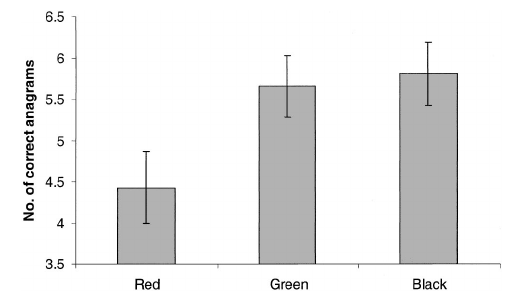
\includegraphics{original}
\end{figure}
Figure~\ref{fig:original} shows that the researchers' results show that red group performed worst with significant difference, whereas green and black group performed similarly.
In order to evaluate the results, researchers used ANCOVA test, where between red and green group, $p < 0.05$ making it statisctically significant. Between green and black group, the
$p$ was higher than $0.81$, not showing difference in performance.
\subsection*{Acquired results}
\begin{figure}[H]
    \centering
    \caption{Black vs red group scores}
    \label{fig:graph1}
    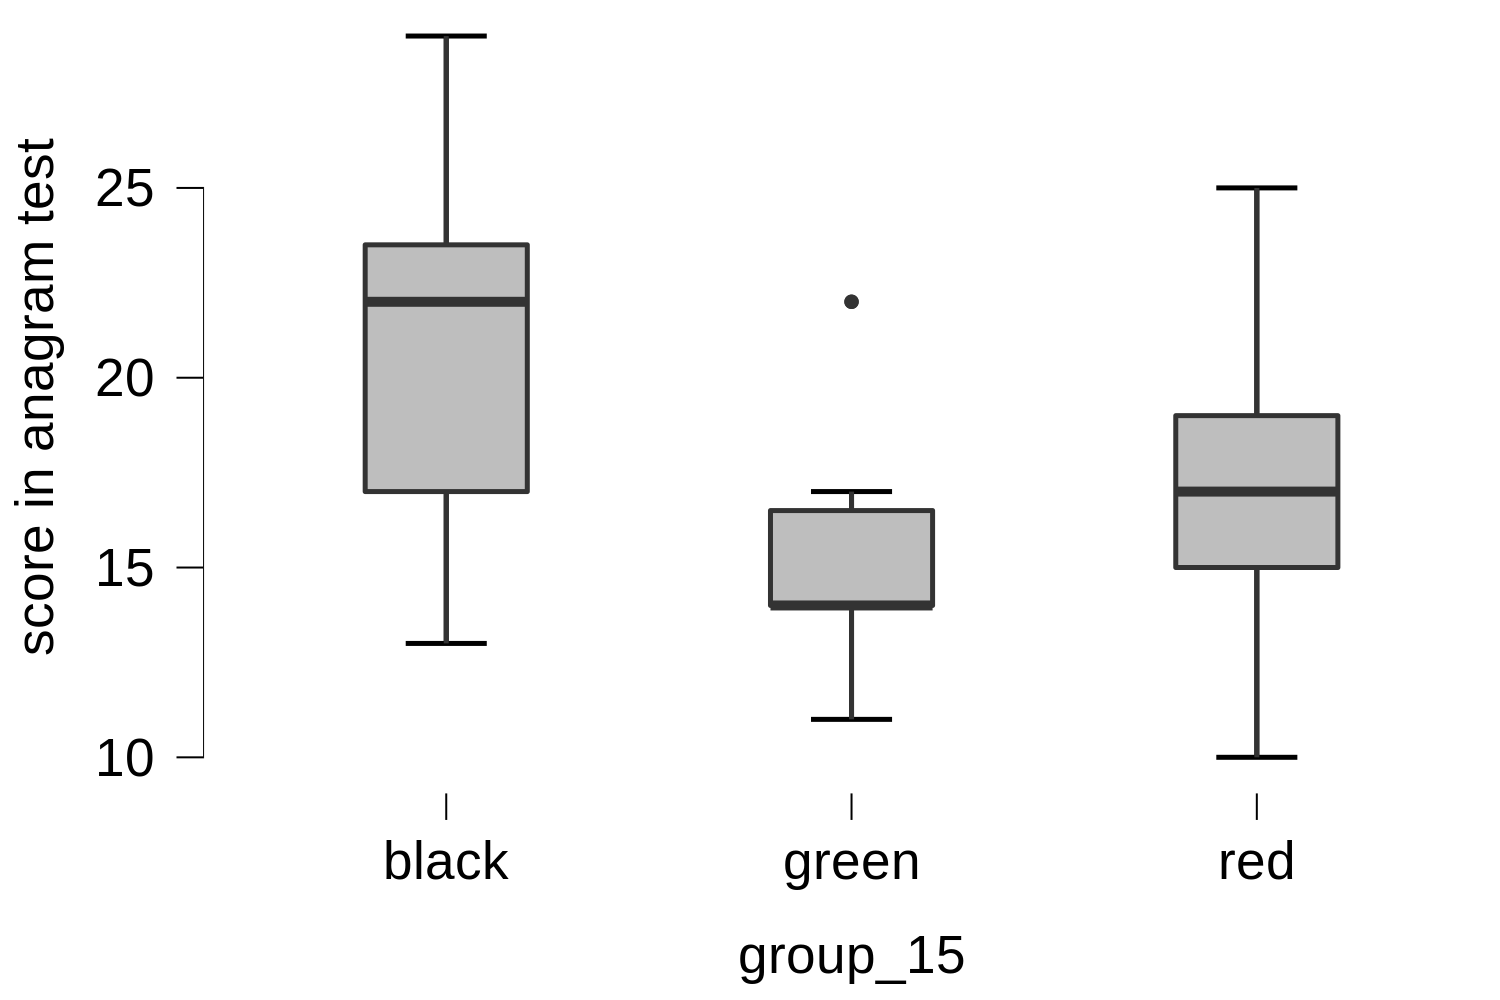
\includegraphics{general}
\end{figure}
\begin{table}[H]
	\centering
	\caption{Descriptive Statistics}
	\label{tab:descriptiveStatistics}
	{
		\begin{tabular}{lrrr}
			\toprule
			\multicolumn{1}{c}{} & \multicolumn{3}{c}{score in anagram test} \\
			\cline{2-4}
			 & black & green & red  \\
			\cmidrule[0.4pt]{1-4}
			Valid & 11 & 10 & 9  \\
			Missing & 0 & 0 & 0  \\
			Mean & 20.636 & 15.500 & 17.222  \\
			Median & 22.000 & 14.000 & 17.000  \\
			Std. Deviation & 4.760 & 3.779 & 4.631  \\
			Minimum & 13.000 & 11.000 & 10.000  \\
			Maximum & 29.000 & 22.000 & 25.000  \\
			\bottomrule
		\end{tabular}
	}
\end{table}
From descrptives, it appears that the hypothesis that red color has negative effect on scores in anagram test checks out, as the mean score of red group was 3 points lower than in 
black group. The caveat is in the green group, which scored the worst, but from the theory it would appear that participants in green group would outperform reds. Standart deviations 
are on roughly the same level in red and black group, whereas in green group it is almost a point lower. In order to check the validity of the results, a series of Mann-Whitney U tests
were performed.
\begin{table}[H]
	\centering
	\caption{Test for red < black}
	\label{tab:br}
	{
		\begin{tabular}{lrrr}
			\toprule
			  & W & df & p  \\
			\cmidrule[0.4pt]{1-4}
			scores & 68.000 &  & 0.084  \\
			\bottomrule
			% \addlinespace[1ex]
			% \multicolumn{4}{p{0.5\linewidth}}{\textit{Note.} For all tests, the alternative hypothesis specifies that group \textit{ b $<$/em> is greater than group <em> r }.} \\
			% \multicolumn{4}{p{0.5\linewidth}}{\textit{Note.} Mann-Whitney U test.} \\
		\end{tabular}
	}
\end{table}
Figure~\ref{tab:br} repesents results for $b > r$ hypothesis and the value of $p$ in Mann-Whitney U test is $0.084$, which is almost 17 times more than significance level, 
making these results not viable for making any conclusions on red having negative effect on cognitive performance.
\begin{table}[H]
	\centering
	\caption{test for b $!=$ color}
	\label{tab:bc}
	{
		\begin{tabular}{lrrr}
			\toprule
			  & W & df & p  \\
			\cmidrule[0.4pt]{1-4}
			scores & 157.500 &  & 0.023  \\
			\bottomrule
			% \addlinespace[1ex]
			% \multicolumn{4}{p{0.5\linewidth}}{\textit{Note.} Mann-Whitney U test.} \\
		\end{tabular}
	}
\end{table}
Test in figure~\ref{tab:bc} check against hypothesis that color has an effect on scores in the test compared to no color group (black). The results show lower, but still 
signifying insignificance $p$ at $0.023$, so not only does the hypothesis checking the impact of specific color on scores appears to be false, but also that any color has any effect 
on the scores.
\section*{Discussion}
The results have not confirmed hypotheses stated before, so the evaluation will be focused on what might have caused the distortion in the results, as the original researchers have shown that 
the red color actually had negative impact on the number of solved anagrams. Considering that the experiment described in this paper was done with no experience in a hectic time, there is no
basis to undermine the validity of the original study. The biggest challenge to overcome in this research was getting participants. Because the experiment was being done when the sophmores were already
learning online, the group from which we could source people shrank to senior year, as they were the only people to legally make consent to an experiment on their own. Because of that fact, we were forced
to take people class by class, and, considering the fact that each class is a collective of people with different predispositions makes for a disruption. The first tested group (black) were people from 
human science profile, so it could be speculated that their word-processing skills were superior to those of bio-chemistry class (red) and math-science group (green), which falls in line with the results, where
people from black group performed best. Other thing questioning itnernal validity was the dispersion in time between testing the groups. Black and red groups were tested within two hours from each other in the morning, 
whereas green group was tested in the afternoon after mock exams, which definetly impacted their cognitive performance. The test itself was done exactly as described in design section, so the disrupting factor is 
definatly sampling of the groups. In order to improve on this research, the people sampled for the test would have to be taken randomly from a bigger set consisting of classes of different profiles, to cancel out 
the differences in word-processing skills. 

\section*{Appendices}
\subsection*{Appendix A : consent form}
\begin{figure}[H]
\centering
    \caption{Consent Form}
    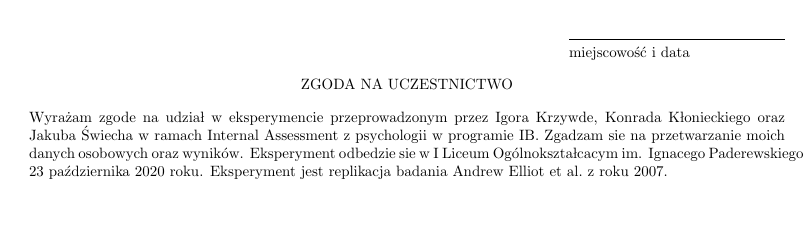
\includegraphics[width=\linewidth]{consent}
\end{figure}
\subsubsection*{Translation}
I consent for participation in an experiment conducted by Igor Krzywda, Konrad Kłoniecki and Jakub Święch as psychology Internal Assessment in IB program. I agree for my personal 
data and my results to be processed. The experiment will take place in I Liceum Ogólnokształcące im. Ignacego Paderewskiego on 23 October 2020. The experiment is a replication of
research done by Andrew Ellion et al. in 2007.
\subsection*{Appendix B : sample test page}
\begin{figure}[H]
\centering
    \caption{Experiment test page}
    
\includegraphics[width=\linewidth]{exp_test}
\end{figure}
\begin{figure}[H]
\centering
    \caption{Experiment practice page}
    
\includegraphics[width=\linewidth]{exp_pr}
\end{figure}
\section*{Sources}
\begin{itemize}
    \item Elliot, A. J., Maier, M. A., Moller, A. C., Friedman, R., \& Meinhardt, J. (2007). Color and psychological functioning: The effect of red on performance attainment. Journal of Experimental Psychology: General, 136(1), 154–168. \url{https://doi.org/10.1037/0096-3445.136.1.154}
    \item D. Rosenstein. (1985, April). Effect of Color of the Environment on Task Performance and Mood of Males and Females with High or Low Scores on the Scholastic Aptitude Test. \url{https://journals.sagepub.com/doi/10.2466/pms.1985.60.2.550}
    \item K. Goldstein (1942). Some experimental observations concerning the influence of colors on the function of the organism. American Journal of Physical Medicine \& Rehabilitation, 1(1), 147–151. \url{https://psycnet.apa.org/record/1942-04745-001}
    \item Wikipedia contributors. (2021, January 4). Yerkes–Dodson law. Wikipedia. \url{https://en.wikipedia.org/wiki/Yerkes-Dodson_law}
\end{itemize}
\end{document}
